\documentclass{article}

\usepackage{booktabs}
\usepackage{tabularx}
\usepackage{graphicx}
\usepackage{float}
\graphicspath{ {./images/} } 
\setlength{\fboxrule}{2pt} % thickness of the border

\title{User Guide\\\progname}

\newcommand{\progname}{McMaster GSA Softball}
\newcommand{\authname}{Derek Li, Damien Cheung, Emma Wigglesworth, \\Jad Haytaoglu, Temituoyo Ugoborogho}

\author{\authname}

\date{}

\begin{document}

\begin{table}[hp]
\caption{Revision History} \label{TblRevisionHistory}
\begin{tabularx}{\textwidth}{llX}
\toprule
\textbf{Date} & \textbf{Developer(s)} & \textbf{Change}\\
\midrule
April 4, 2025 & Derek Li & Finalized User Guide\\
... & ... & ...\\
\bottomrule
\end{tabularx}
\end{table}

\newpage

\maketitle

\tableofcontents

\newpage

\section{Introduction}
The McMaster GSA Softball Platform User Guide provides step-by-step instructions for players to register for the league, join teams, and manage their participation. This guide covers key actions such as viewing schedules, checking game results, and updating player profiles. Whether you're a new player or a returning member, this document will help you navigate the platform with ease

\section{Getting Started: Signing Up}
When new users visit the McMaster GSA Softball Platform, they will see the login screen. To create an account, follow these steps:

\begin{enumerate}
    \item \textbf{Go to the Login Page} – Open the platform’s website and navigate to the login screen.
    \item \textbf{Click "Sign Up"} – Below the login fields, select the option to create a new account.
    \item \textbf{Enter Your Information} – Fill in the required fields:
    \begin{itemize}
        \item \textbf{First Name}
        \item \textbf{Last Name}
        \item \textbf{Email Address}
        \item \textbf{Password}
    \end{itemize}
    \item \textbf{Log In} – Return to the login page, enter your email and password, and access your account.
\end{enumerate}

\section{Overview of Features and Functionality}

The platform is designed to provide users with an intuitive, self-service experience, allowing players and commissioners to manage their activities seamlessly. With a user-friendly interface, players can easily register, manage, and modify their teams, while commissioners can efficiently oversee and manage the entire season. Below are the key features and functionalities of the platform.

\subsection{User Features}

\begin{itemize}
    \item \textbf{Create and Manage Teams:} Players can easily create their own teams by registering through the home page. The registering player automatically becomes the captain of the team. This allows captains to invite new members and coordinate games using the rescheduling system.
    \item \textbf{Join a Team:} Players wishing to join a team must be invited by a team captain. Captains can browse through the list of players and send out invitations to join their team. Once the player accepts the invitation, they will be added to the team’s roster. This ensures that only players personally invited by the captain can join a team, keeping the process streamlined and controlled.
    \item \textbf{Leave a Team:} Players can leave a team at any time through the team management page. If a player decides to leave, they can rejoin another team through invitation. The platform ensures that leaving a team does not affect other players or the team’s standing.
    \item \textbf{View Team and Season Progress:} Players have access to view their team’s progress, upcoming match schedules, and results. Additionally, they can keep track of the overall season standings, which helps players stay informed and motivated throughout the competition.
\end{itemize}

\subsection{Commissioner Features}

\begin{itemize}
    \item \textbf{Manage Seasons:} Commissioners have full control over season management. They can open, launch, and archive seasons, manage registered teams and their preferences, and set important deadlines for team registration. These functionalities ensure each season runs smoothly and on schedule.
    \item \textbf{Approve/Reject Team Registrations:} Commissioners can review team registrations to ensure compliance with platform rules and waiver consent. Commissioners can approve teams at their discretion based on whether the team has paid their cash fee and overall eligibility. Commissioners can move teams between divisions if needed, which helps maintain a fair and competitive environment.
    \item \textbf{Create and Manage Announcements:} Commissioners can easily create, update, and remove announcements to keep teams and players informed. Whether it’s deadline reminders, rule updates, or general season info, announcements ensure everyone stays in the loop.
    \item \textbf{Intuitive, Easy-to-Use Interface:} The platform is designed for efficiency and ease of use. An intuitive dashboard gives commissioners quick access to team management, registration data, progress tracking, and announcements in just a few clicks.
\end{itemize}

\noindent Overall, the platform empowers players to manage their teams and join or leave as needed, while giving commissioners all the tools required to efficiently manage the season. The ease of use for both players and commissioners ensures that everyone can focus on enjoying the season and the competition, without the platform getting in the way.

\section{Player's Manual}
\subsection{Register Team}
Navigate to the home page to register your team for the desired season. The registering player will become the captain of their team. Keep in mind, accounts can only belong on one team per season. Ongoing seasons can also be viewed here.

\begin{figure}[H]
    \centering
    \fbox{
\includegraphics[width=1\textwidth]{registerteam1.png}}
    \caption{Navigate to home view}
\end{figure}
\begin{figure}[H]
    \fbox{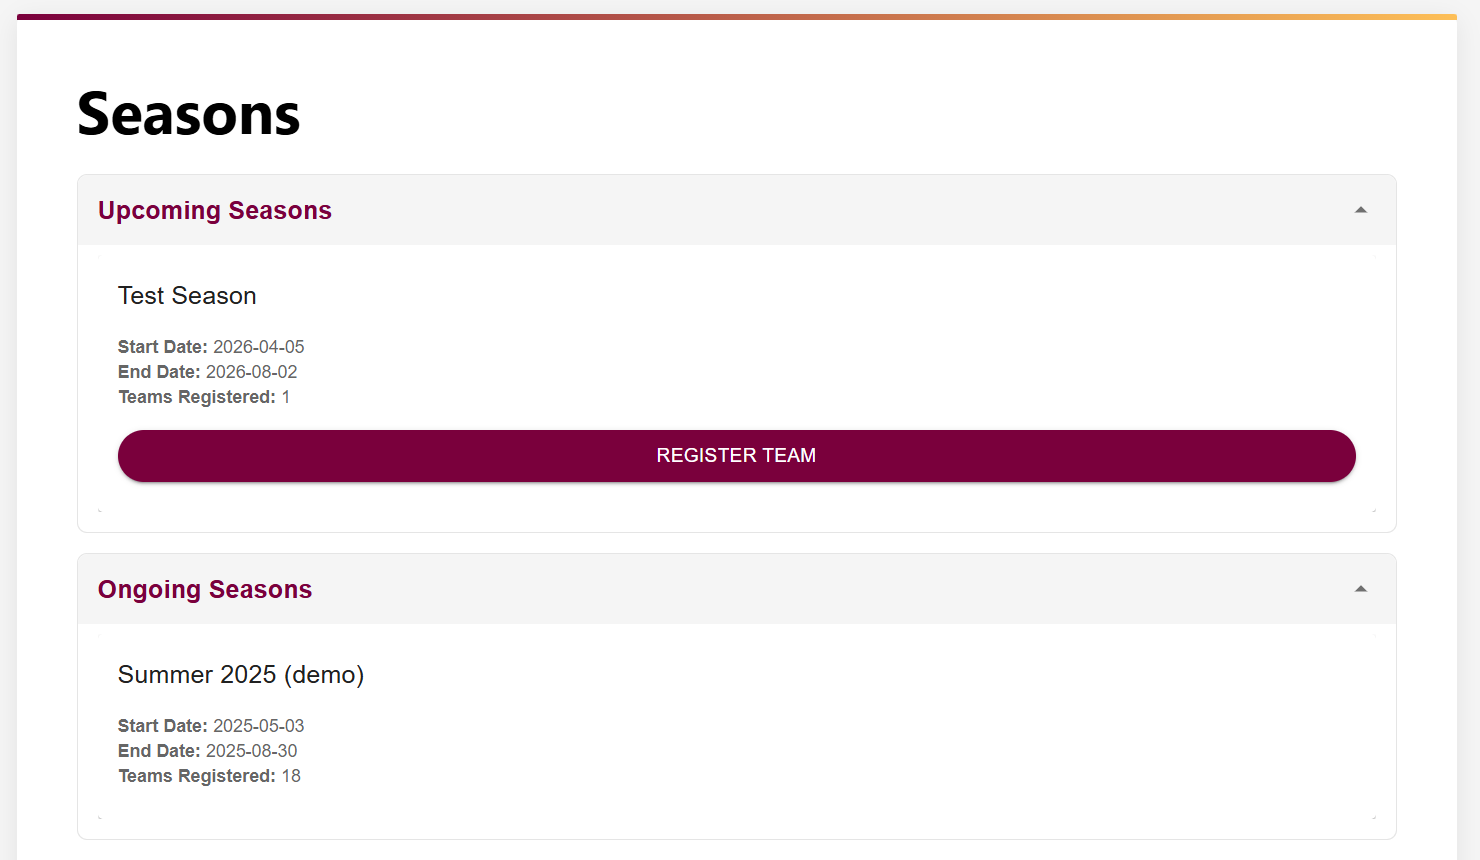
\includegraphics[width=1\textwidth]{registerteam2.png}}
    \caption{Register team under upcoming seasons}
\end{figure}

\subsection{Accept Team Invite}
Players can accept team invites by navigating to the "My Team" page. You will see all team invitations there. Click "Click to Accept" to join the team. Each account can only be on one team per season.

\begin{figure}[H]
    \centering
    \fbox{
\includegraphics[width=1\textwidth]{acceptinvite1.png}}
    \caption{Navigate to my team view}
\end{figure}

\begin{figure}[H]
    \centering
    \fbox{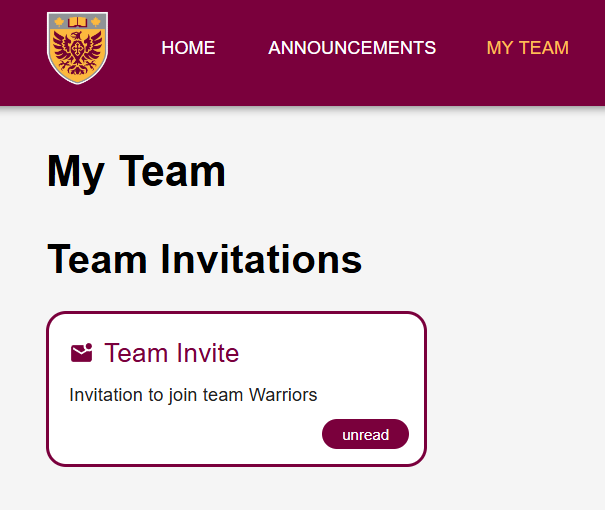
\includegraphics[width=1\textwidth]{acceptinvite2.png}}
    \caption{Click to accept team invite}
\end{figure}

\subsection{Team Roster and Contact}
Navigate to the "My Team" page and scroll down. Here, the team roster includes the email contact for all your teammates. Phone number is optional.

\begin{figure}[H]
    \centering
    \fbox{
\includegraphics[width=1\textwidth]{team1.png}}
    \caption{Navigate to my team view}
\end{figure}

\begin{figure}[H]
    \centering
    \fbox{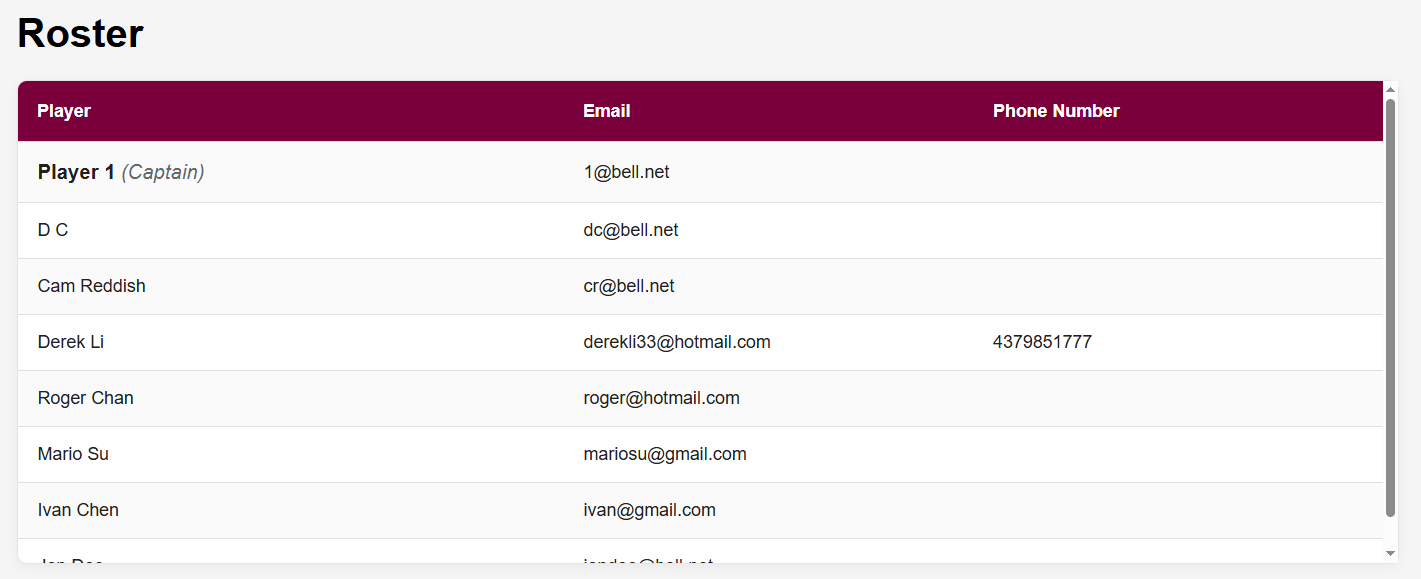
\includegraphics[width=1\textwidth]{team2.png}}
    \caption{Scroll down to view team roster and information}
\end{figure}

\subsection{Schedule}
Navigate to the schedule page to view your games. The schedule page offers multiple views:

\begin{itemize}
    \item \textbf{Weekly Schedule}: Displays games in a weekly format.
    \item \textbf{Team Schedule}: Displays games for your team in a monthly format.
    \item \textbf{League Schedule}: Displays all games in your division in a monthly format.
\end{itemize}

\begin{figure}[H]
    \centering
    \fbox{
\includegraphics[width=1\textwidth]{schedule1.png}}
    \caption{Navigate to Schedule View}
\end{figure}

\begin{figure}[H]
    \centering
    \fbox{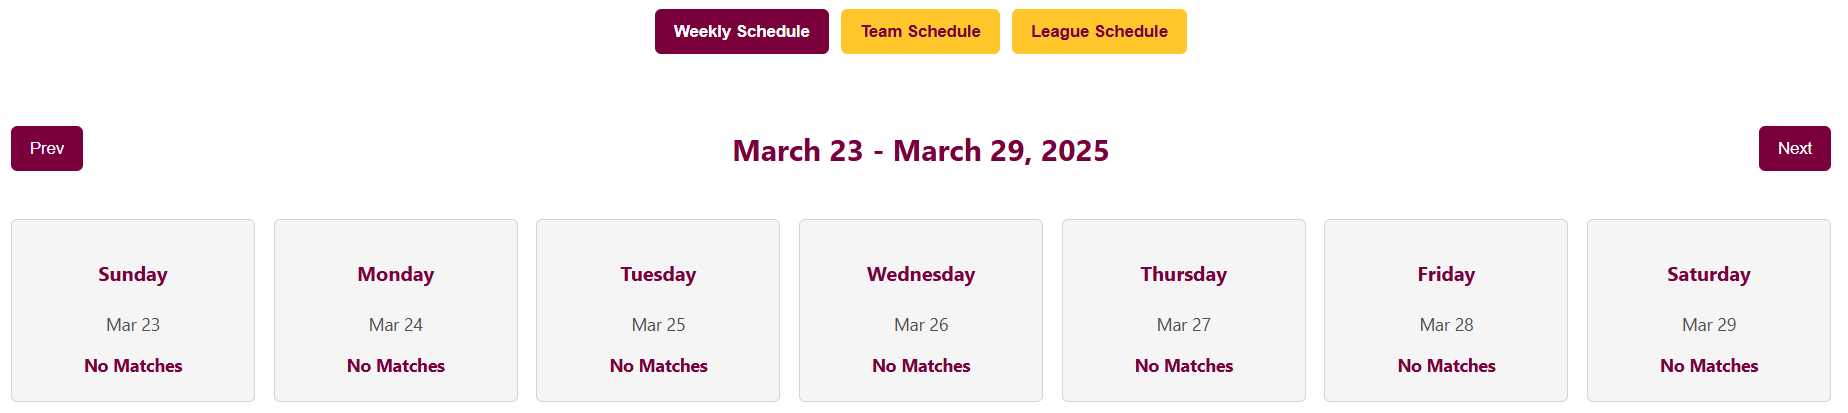
\includegraphics[width=1\textwidth]{schedule2.png}}
    \caption{Weekly Schedule View}
\end{figure}

\begin{figure}[H]
    \centering
    \fbox{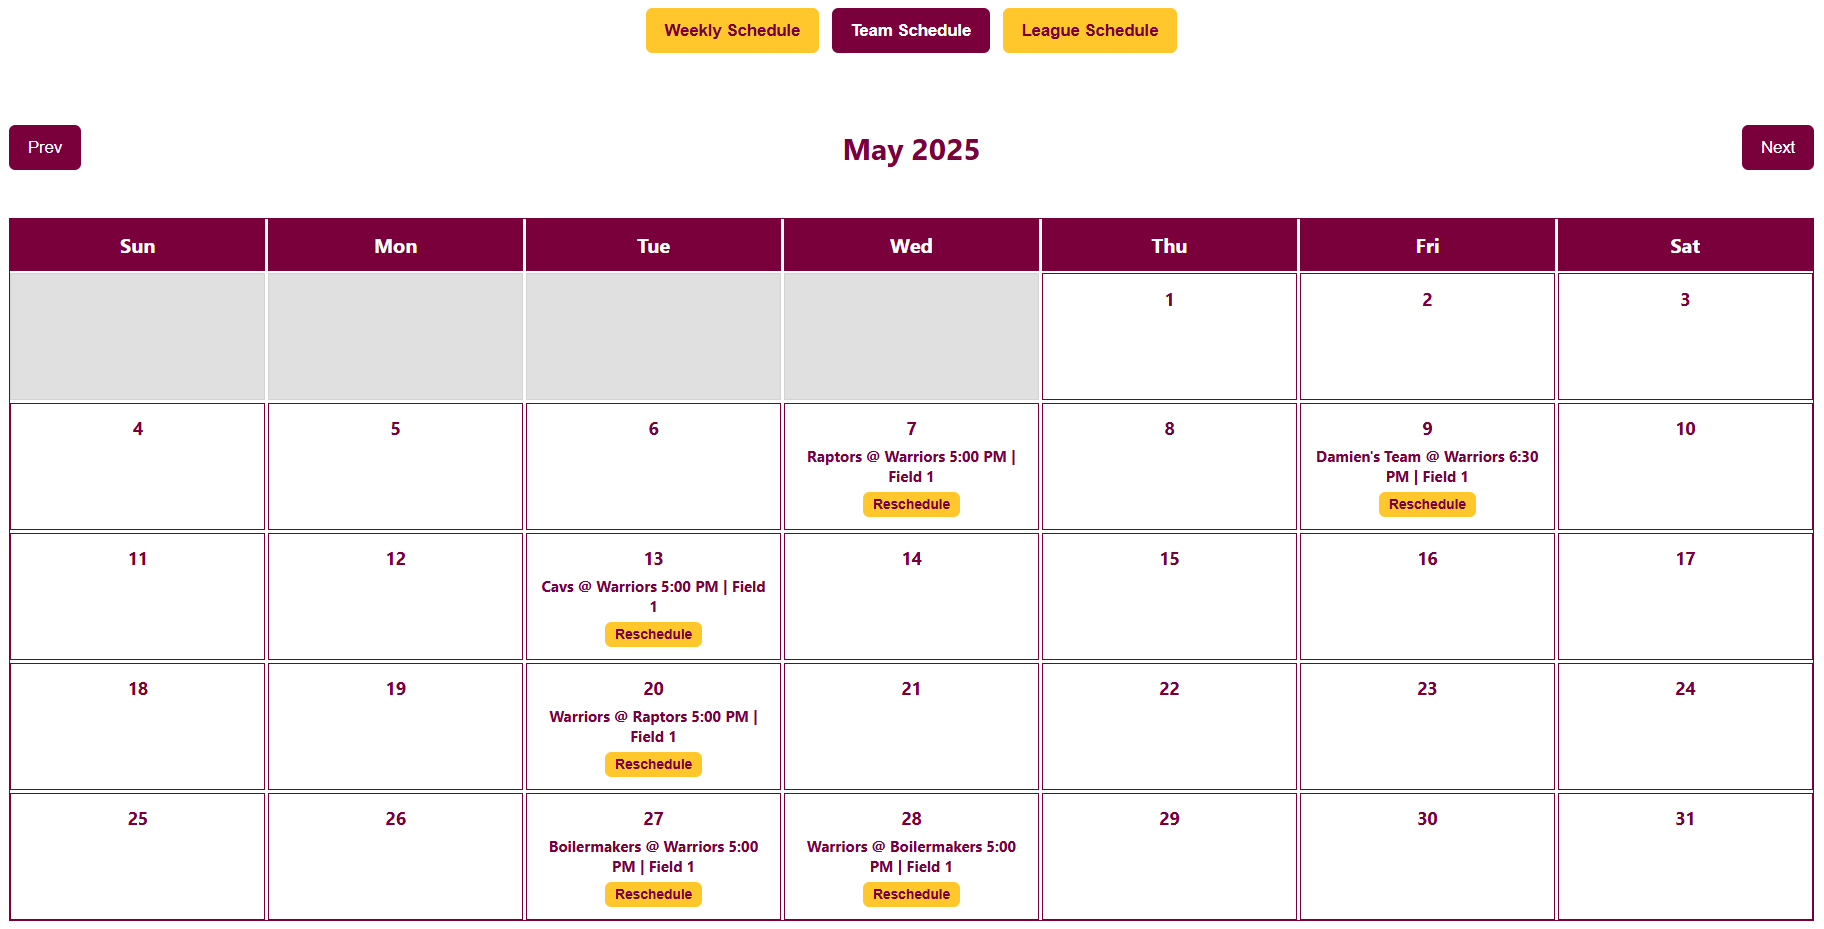
\includegraphics[width=1\textwidth]{schedule3.png}}
    \caption{Team Schedule View}
\end{figure}

\begin{figure}[H]
    \centering
    \fbox{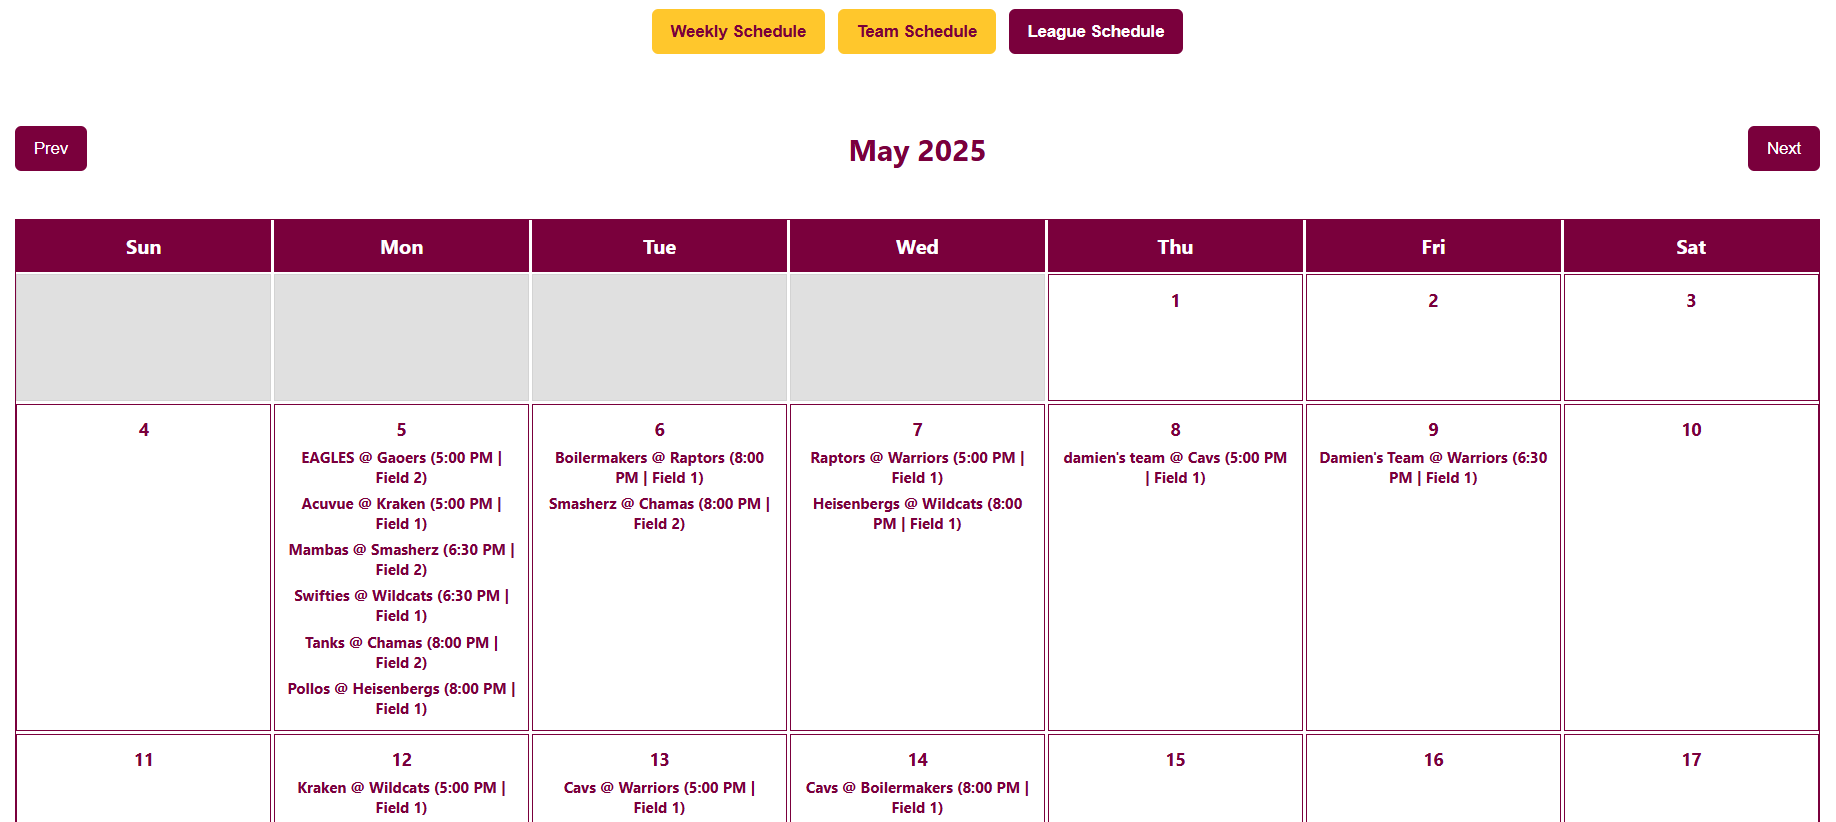
\includegraphics[width=1\textwidth]{schedule4.png}}
    \caption{League Schedule View}
\end{figure}

\subsection{Edit Profile}
Navigate to the profile page to edit your profile information. Click "Edit" and proceed to make your desired changes. Once you're done, click "Done" to finalize changes.

\begin{figure}[H]
    \centering
    \fbox{
\includegraphics[width=1\textwidth]{profile1.png}}
    \caption{Navigate to profile view}
\end{figure}

\begin{figure}[H]
    \centering
    \fbox{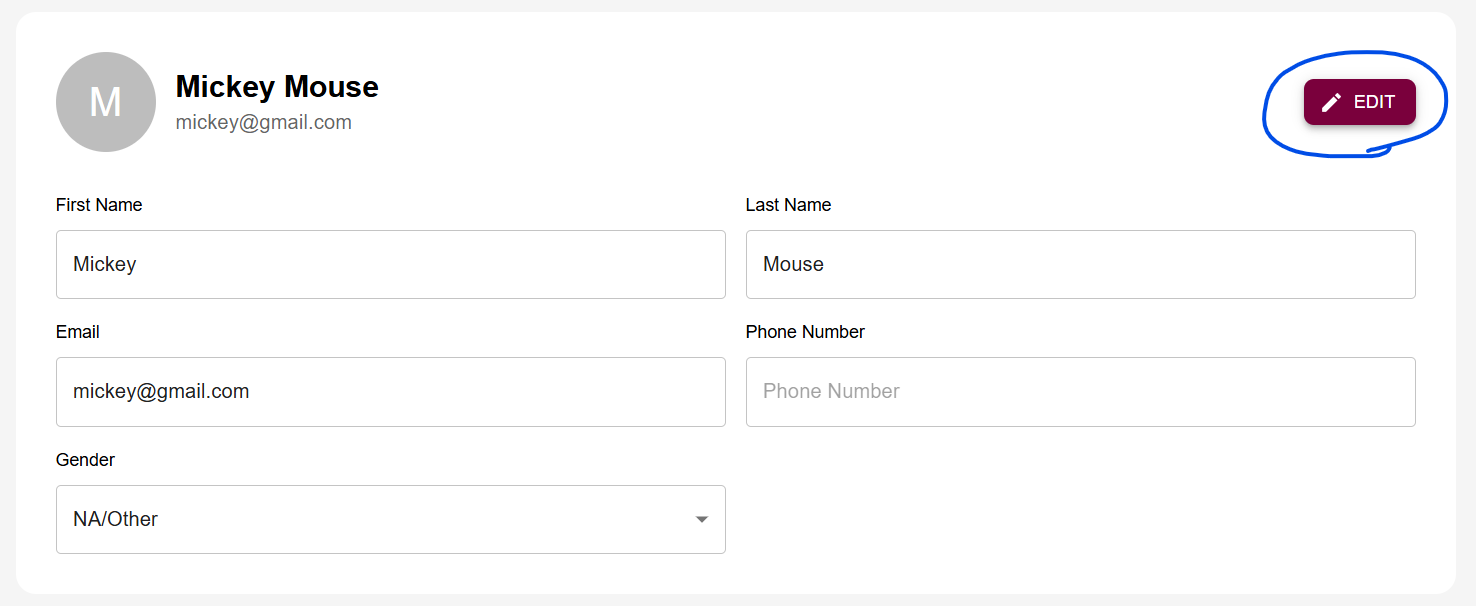
\includegraphics[width=1\textwidth]{profile2.png}}
    \caption{Press edit to enable editing mode}
\end{figure}

\begin{figure}[H]
    \centering
    \fbox{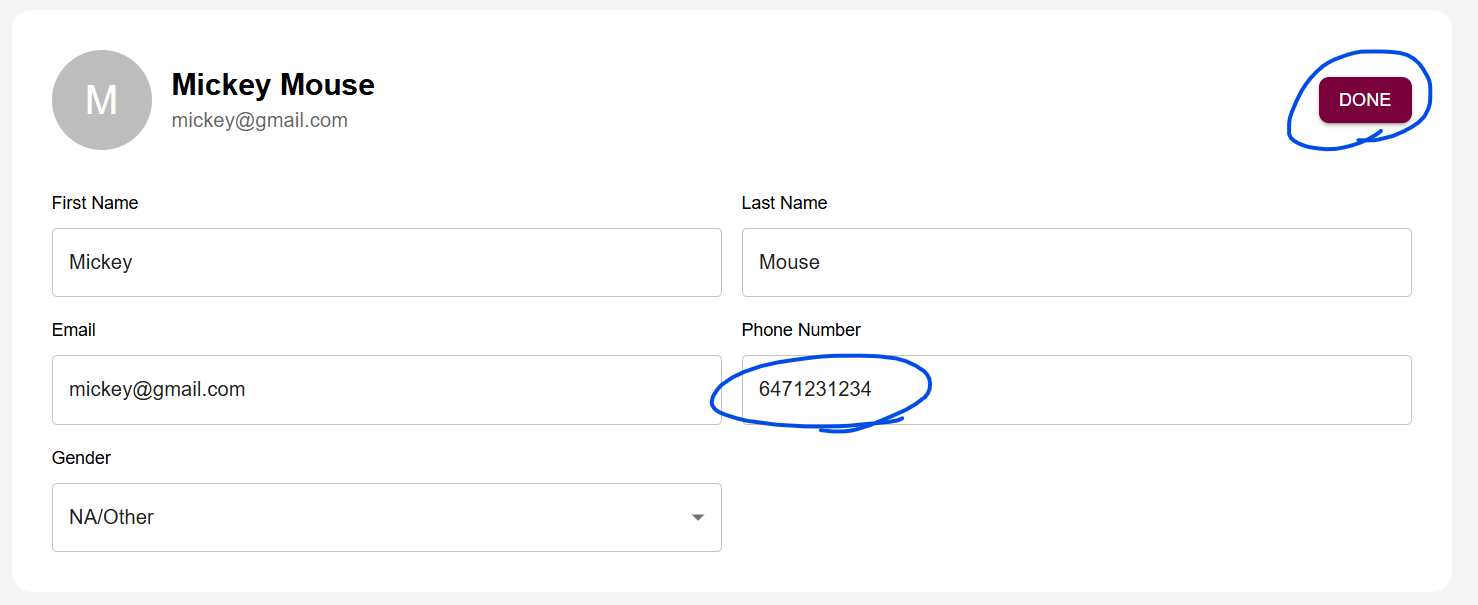
\includegraphics[width=1\textwidth]{profile3.png}}
    \caption{Press done to confirm changes}
\end{figure}

\section{Captain's Manual}
\subsection{Invite Players}
Captains can invite players by navigating to the "Invite Players" button located on the "My Team" page. Select "Invite Players" to open the list of players, and click "Invite to Team" to invite them.

\begin{figure}[H]
    \centering
    \fbox{
\includegraphics[width=1\textwidth]{inviteplayers1.png}}
    \caption{Navigate to my team view}
\end{figure}

\begin{figure}[H]
    \centering
    \fbox{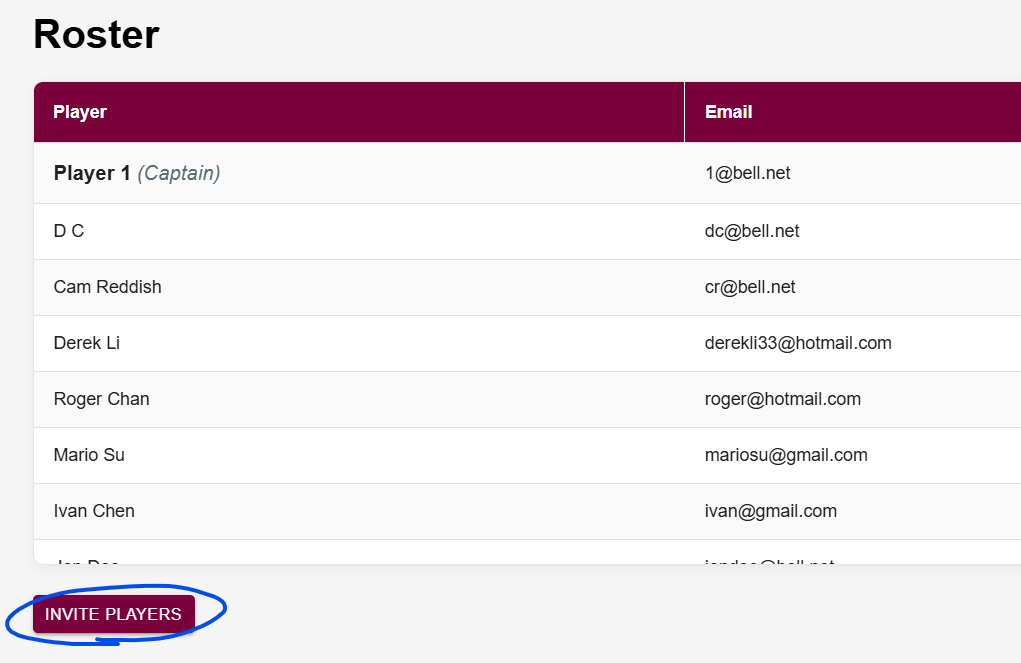
\includegraphics[width=1\textwidth]{inviteplayers2.png}}
    \caption{Press invite players underneath the team roster}
\end{figure}

\begin{figure}[H]
    \centering
    \fbox{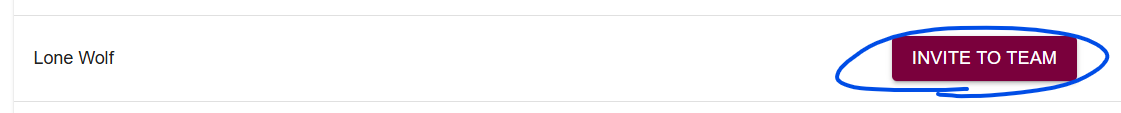
\includegraphics[width=1\textwidth]{inviteplayers3.png}}
    \caption{Press invite to team to invite the following player}
\end{figure}

\subsection{Submit Scores}
The captain of the winning team is responsible for submitting the game score. To do so, navigate to the "My Team" page, find the schedule, fill out the scores, and click "Submit Score."

\begin{figure}[H]
    \centering
    \fbox{
\includegraphics[width=1\textwidth]{submitscores1.png}}
    \caption{Navigate to my team view}
\end{figure}

\begin{figure}[H]
    \centering
    \fbox{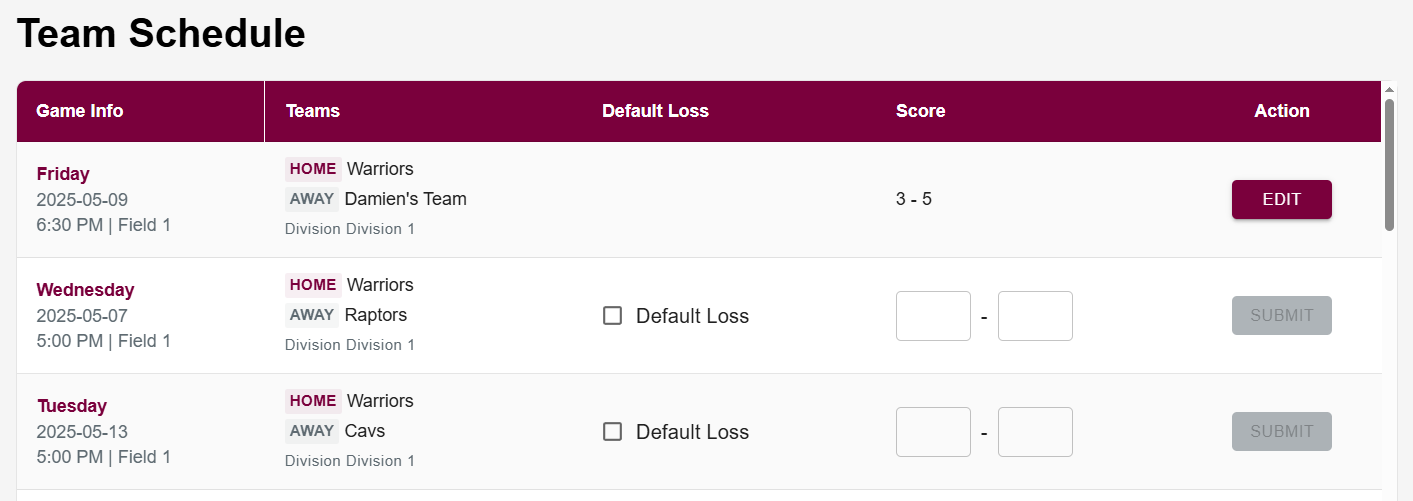
\includegraphics[width=1\textwidth]{submitscores2.png}}
    \caption{Fill out the score and press submit}
\end{figure}

\subsection{Request to Reschedule Games}
Captains are responsible for rescheduling games. Navigate to the schedule page, and select the "Reschedule" button next to the game you wish to reschedule.

\begin{figure}[H]
    \centering
    \fbox{
\includegraphics[width=1\textwidth]{reschedule1.png}}
    \caption{Navigate to schedule view}
\end{figure}

\begin{figure}[H]
    \centering
    \fbox{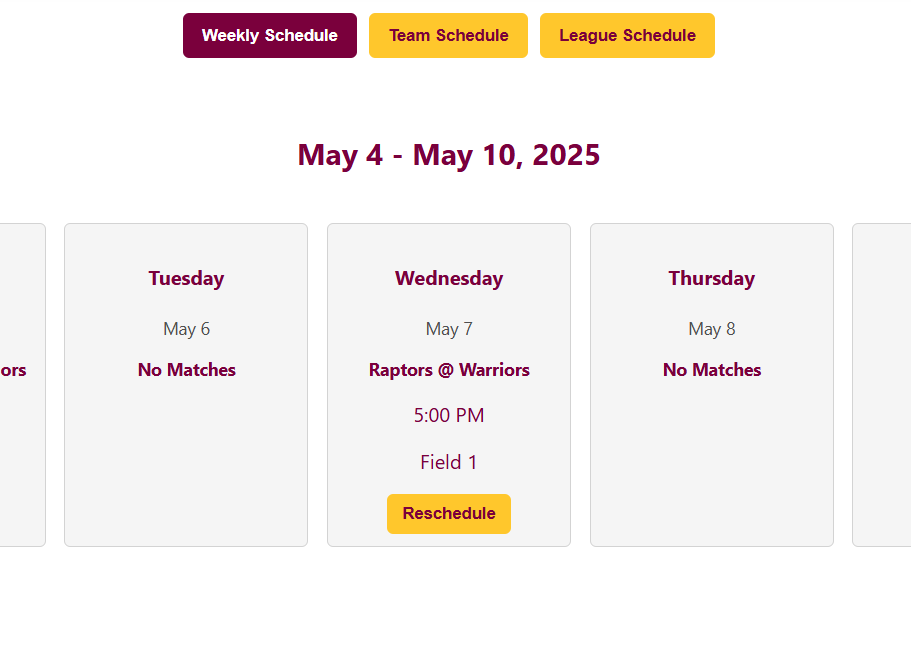
\includegraphics[width=1\textwidth]{reschedule2.png}}
    \caption{Press reschedule on the game you wish to reschedule}
\end{figure}

\begin{figure}[H]
    \centering
    \fbox{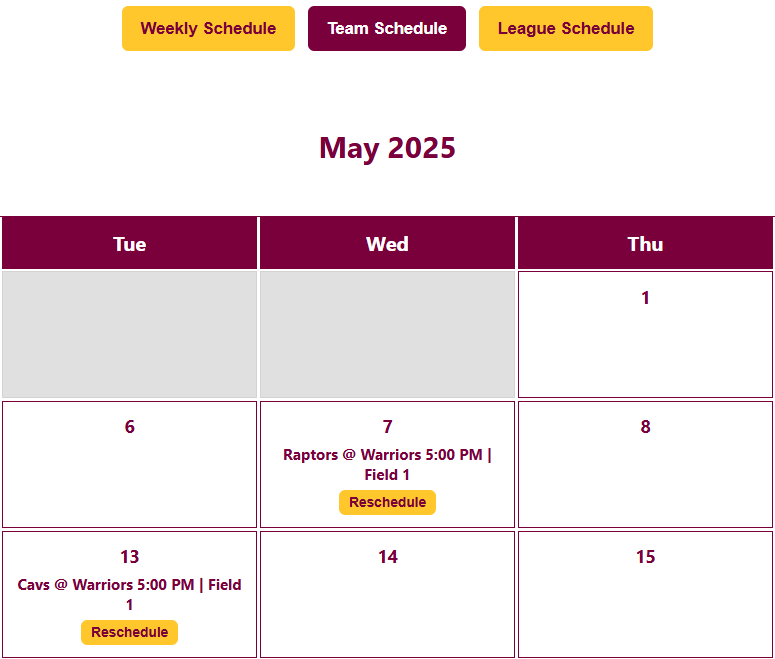
\includegraphics[width=1\textwidth]{reschedule3.png}}
    \caption{Alternatively, you can also find the reschedule button in other views}
\end{figure}

\begin{figure}[H]
    \centering
    \fbox{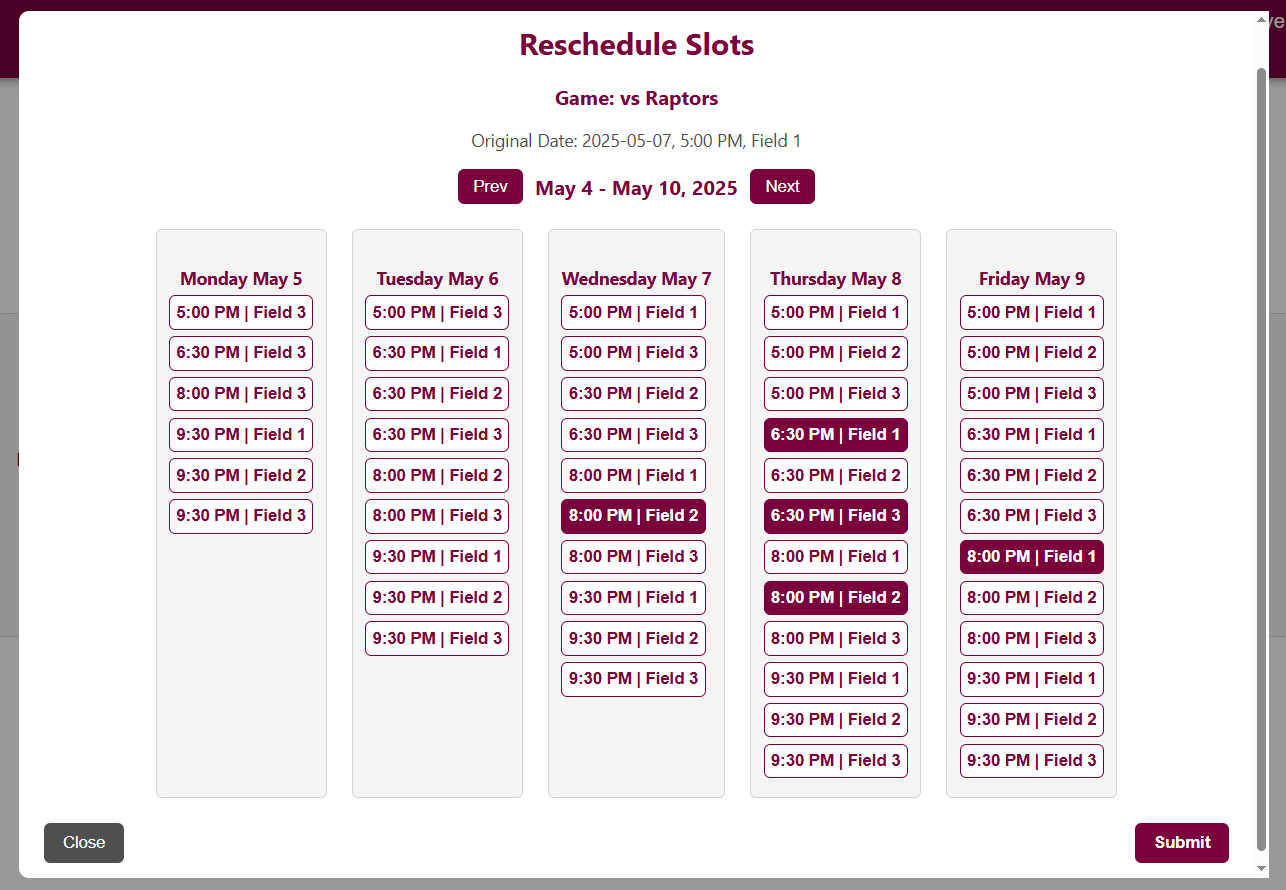
\includegraphics[width=1\textwidth]{reschedule4.png}}
    \caption{Select the time you would like to reschedule to and click submit}
\end{figure}

\subsection{Respond to Reschedule Requests}
Captains can respond to reschedule requests in the "My Team" page under the scheduling notifications section.

\begin{figure}[H]
    \centering
    \fbox{
\includegraphics[width=1\textwidth]{respond1.png}}
    \caption{Navigate to my team page}
\end{figure}

\begin{figure}[H]
    \centering
    \fbox{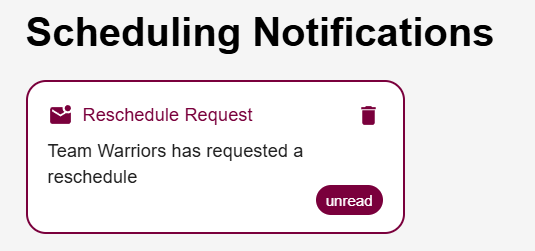
\includegraphics[width=1\textwidth]{respond2.png}}
    \caption{Read reschedule requests under scheduling notifications}
\end{figure}

\begin{figure}[H]
    \centering
    \fbox{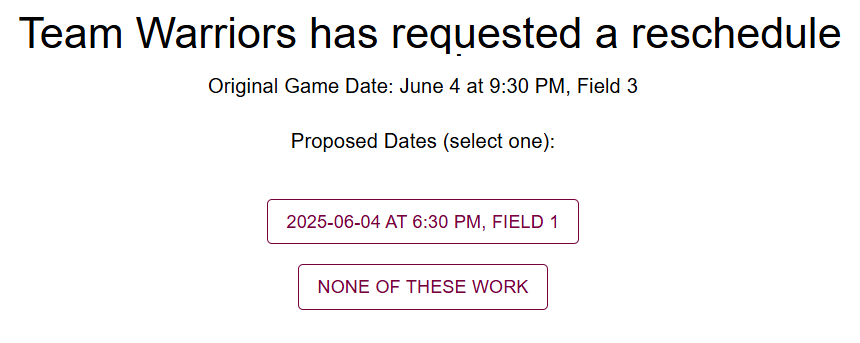
\includegraphics[width=1\textwidth]{respond3.png}}
    \caption{Here, you can view the proposed dates from the other team}
\end{figure}

\begin{figure}[H]
    \centering
    \fbox{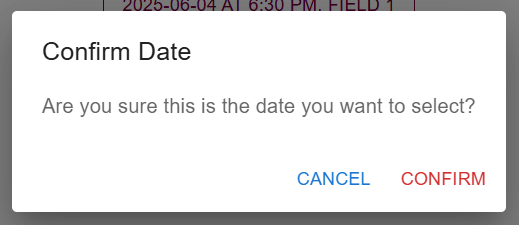
\includegraphics[width=1\textwidth]{respond4.png}}
    \caption{You can accept one of the proposed dates}
\end{figure}


\begin{figure}[H]
    \centering
    \fbox{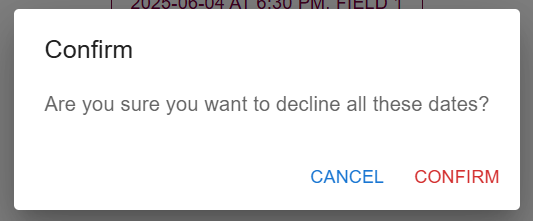
\includegraphics[width=1\textwidth]{respond5.png}}
    \caption{You can also choose to decline all the proposed dates}
\end{figure}

\section{Commissioner's Manual}
\subsection{Announcements}
The commissioner can create, edit, and delete announcements, a form of communication to the users on the platform.

\begin{figure}[H]
    \centering
    \fbox{
\includegraphics[width=1\textwidth]{announcements1.png}}
    \caption{Navigate to the announcements view}
\end{figure}

\begin{figure}[H]
    \centering
    \fbox{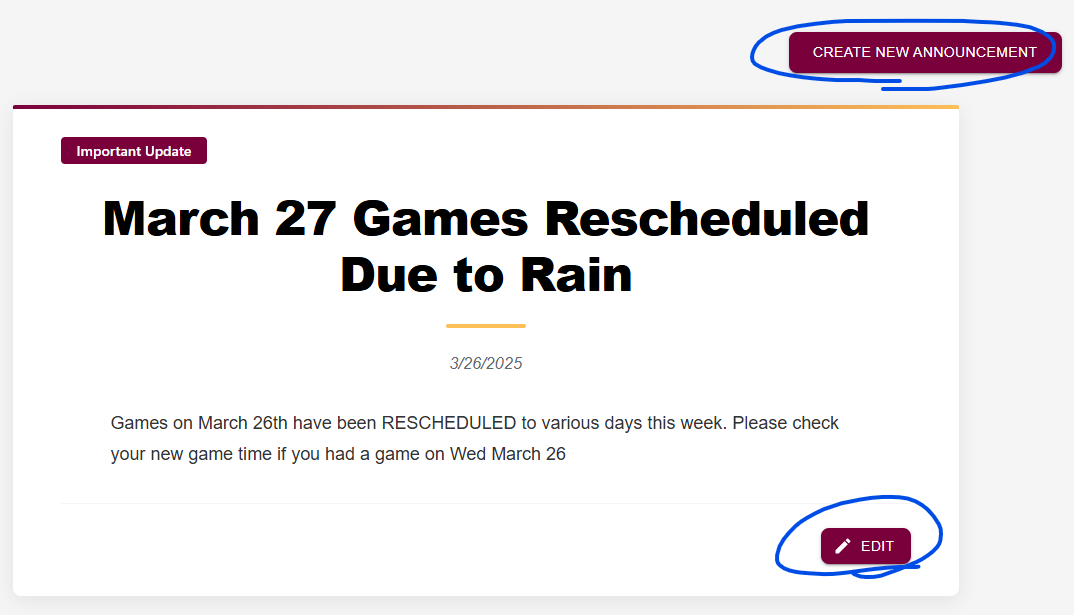
\includegraphics[width=1\textwidth]{announcements2.png}}
    \caption{Here, you can create new announcement or edit existing ones}
\end{figure}

\begin{figure}[H]
    \centering
    \fbox{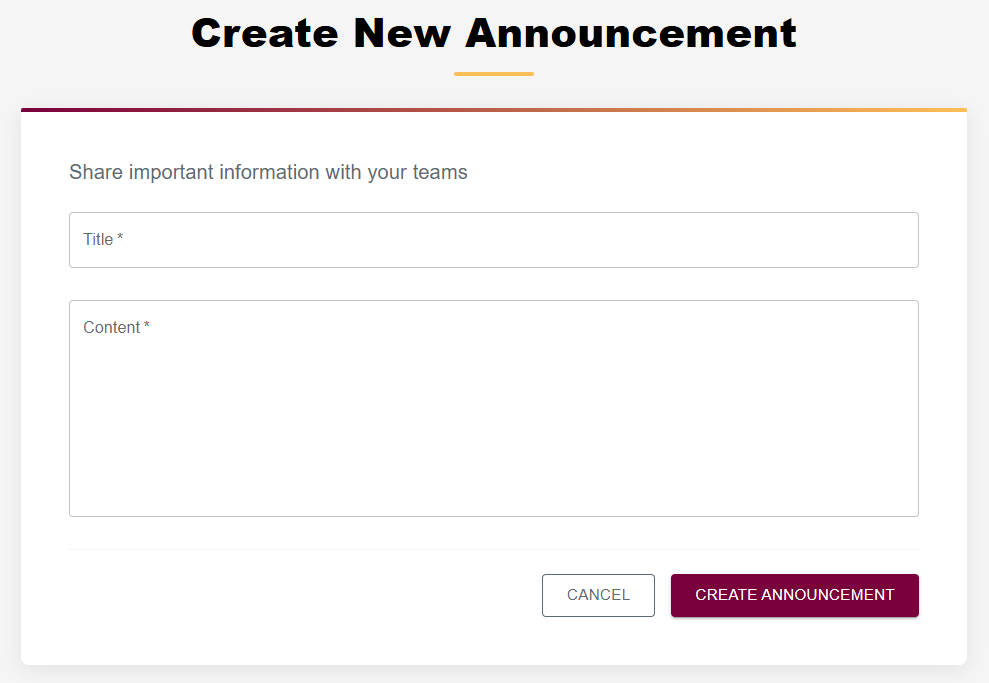
\includegraphics[width=1\textwidth]{announcements3.png}}
    \caption{Fill out the announcement and click create announcement}
\end{figure}

\begin{figure}[H]
    \centering
    \fbox{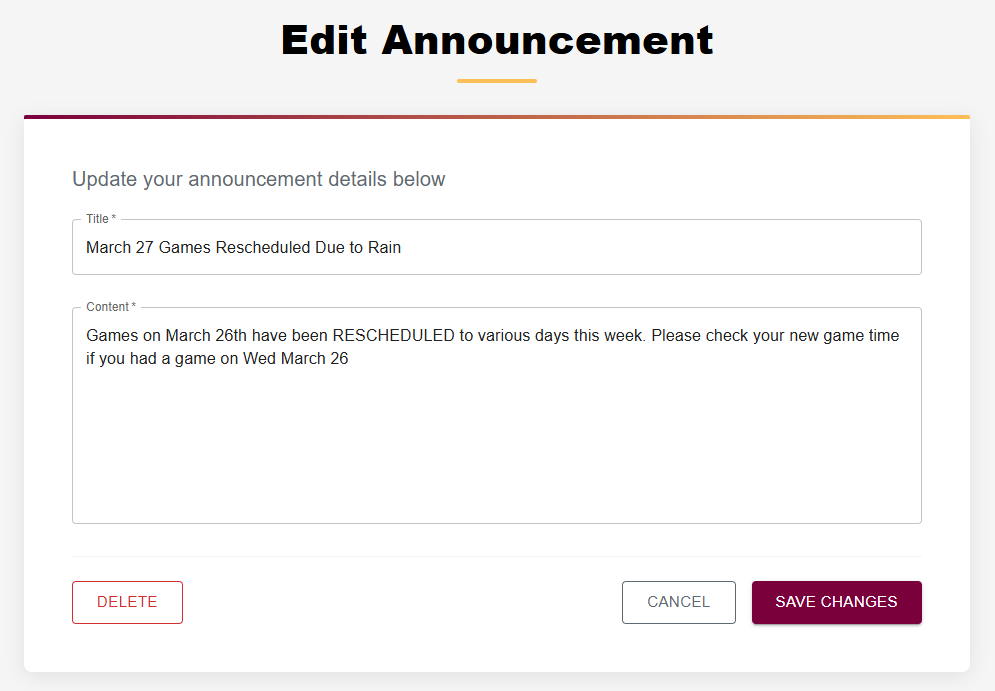
\includegraphics[width=1\textwidth]{announcements4.png}}
    \caption{Existing announcements can be deleted or edited}
\end{figure}

\subsection{Manage Seasons}
The commissioner can create new seasons and delete seasons that are no longer needed.

\begin{figure}[H]
    \centering
    \fbox{
\includegraphics[width=1\textwidth]{seasons1.png}}
    \caption{Navigate to the manage view}
\end{figure}

\begin{figure}[H]
    \centering
    \fbox{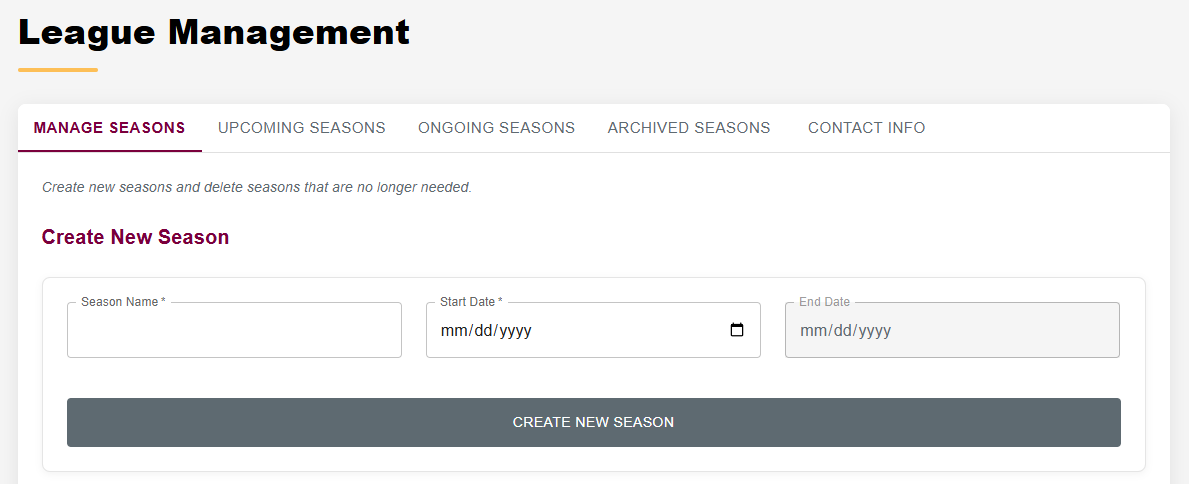
\includegraphics[width=1\textwidth]{seasons2.png}}
    \caption{In the manage seasons tab, you can fill out the season name and start date}
\end{figure}

\begin{figure}[H]
    \centering
    \fbox{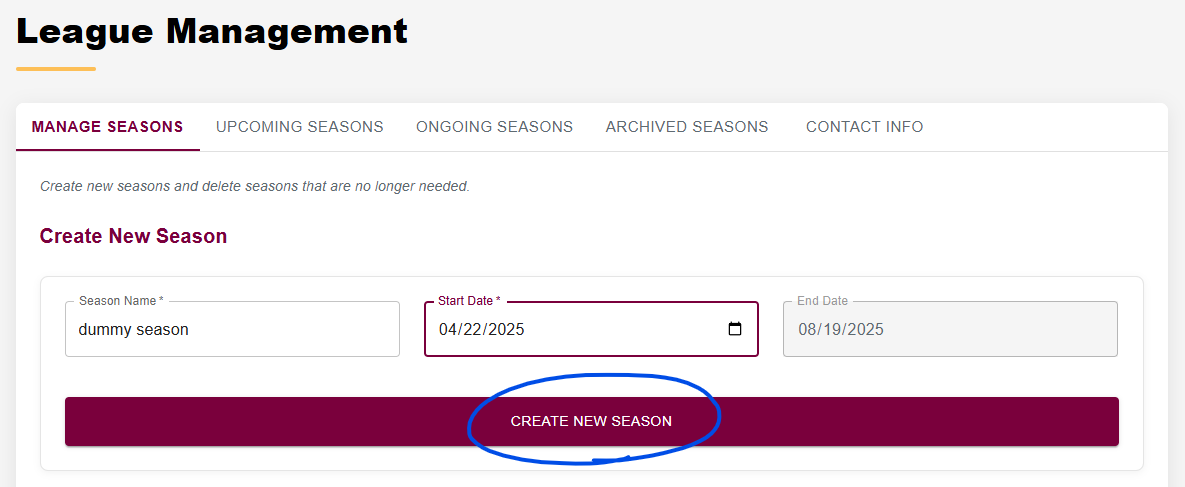
\includegraphics[width=1\textwidth]{seasons3.png}}
    \caption{Once filled out, click create new season}
\end{figure}

\begin{figure}[H]
    \centering
    \fbox{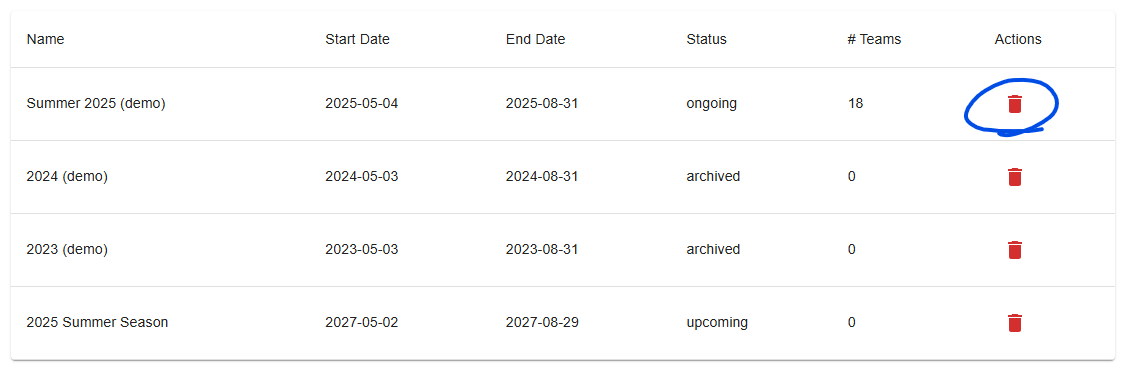
\includegraphics[width=1\textwidth]{seasons4.png}}
    \caption{You can view all seasons below and choose to delete them if needed}
\end{figure}

\subsection{Upcoming Seasons}
The commissioner can manage and launch seasons that are currently open for registration. Seasons will automatically launch on the start date.

\begin{figure}[H]
    \centering
    \fbox{
\includegraphics[width=1\textwidth]{upcomingseasons1.png}}
    \caption{Navigate to the manage view}
\end{figure}

\begin{figure}[H]
    \centering
    \fbox{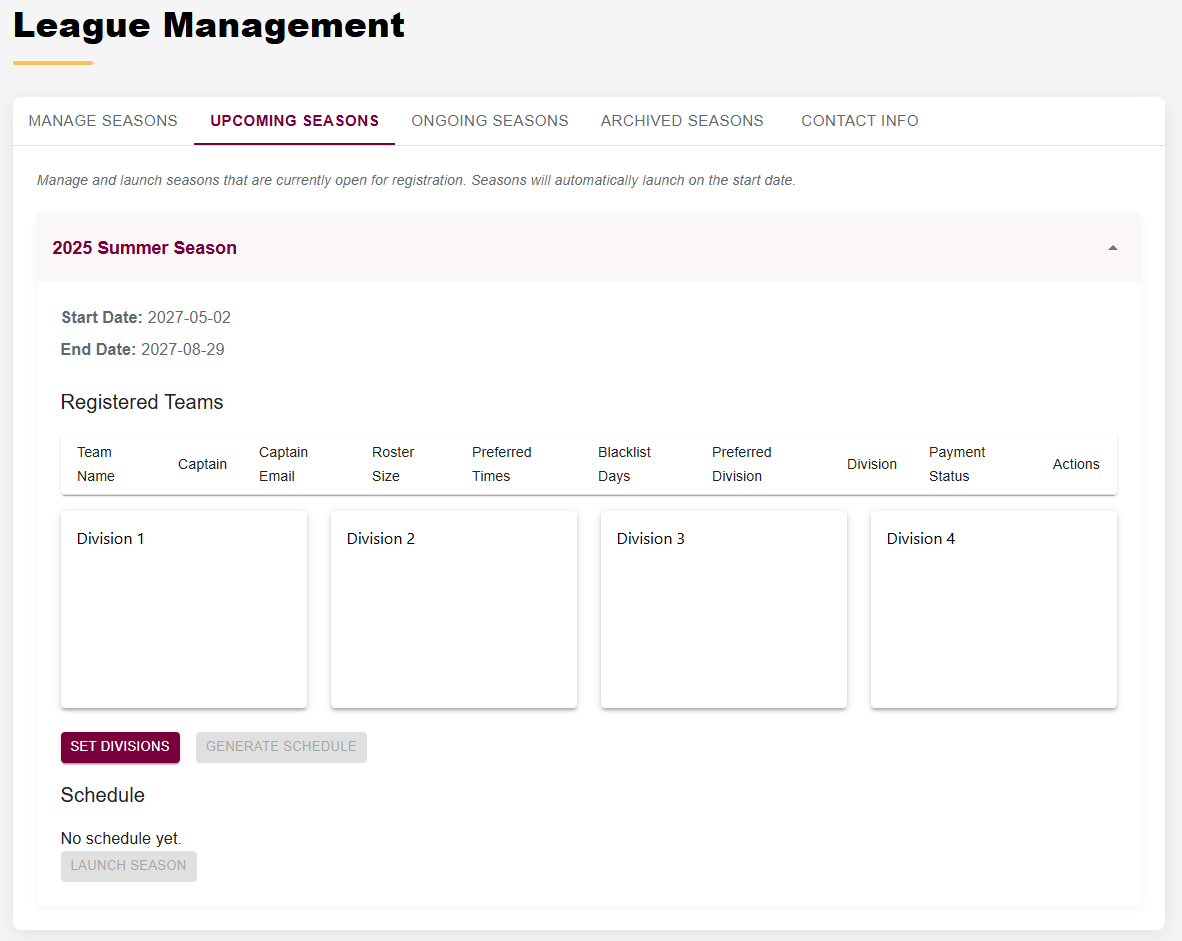
\includegraphics[width=1\textwidth]{upcomingseasons2.png}}
    \caption{In the upcoming seasons tab, teams can be dragged and moved into other divisions}
\end{figure}

\begin{figure}[H]
    \centering
    \fbox{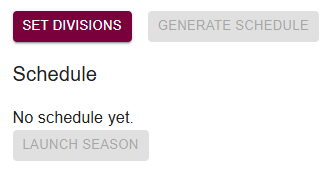
\includegraphics[width=1\textwidth]{upcomingseasons3.png}}
    \caption{When done, click set division and generate schedule to launch schedule. Select launch season to launch the season with the finalized schedule}
\end{figure}

\subsection{Ongoing Seasons}
The commissioner can input scores if needed and view the schedules and results of ongoing seasons. Seasons will be automatically archived after the end date.

\begin{figure}[H]
    \centering
    \fbox{
\includegraphics[width=1\textwidth]{ongoingseasons1.png}}
    \caption{Navigate to the manage view}
\end{figure}

\begin{figure}[H]
    \centering
    \fbox{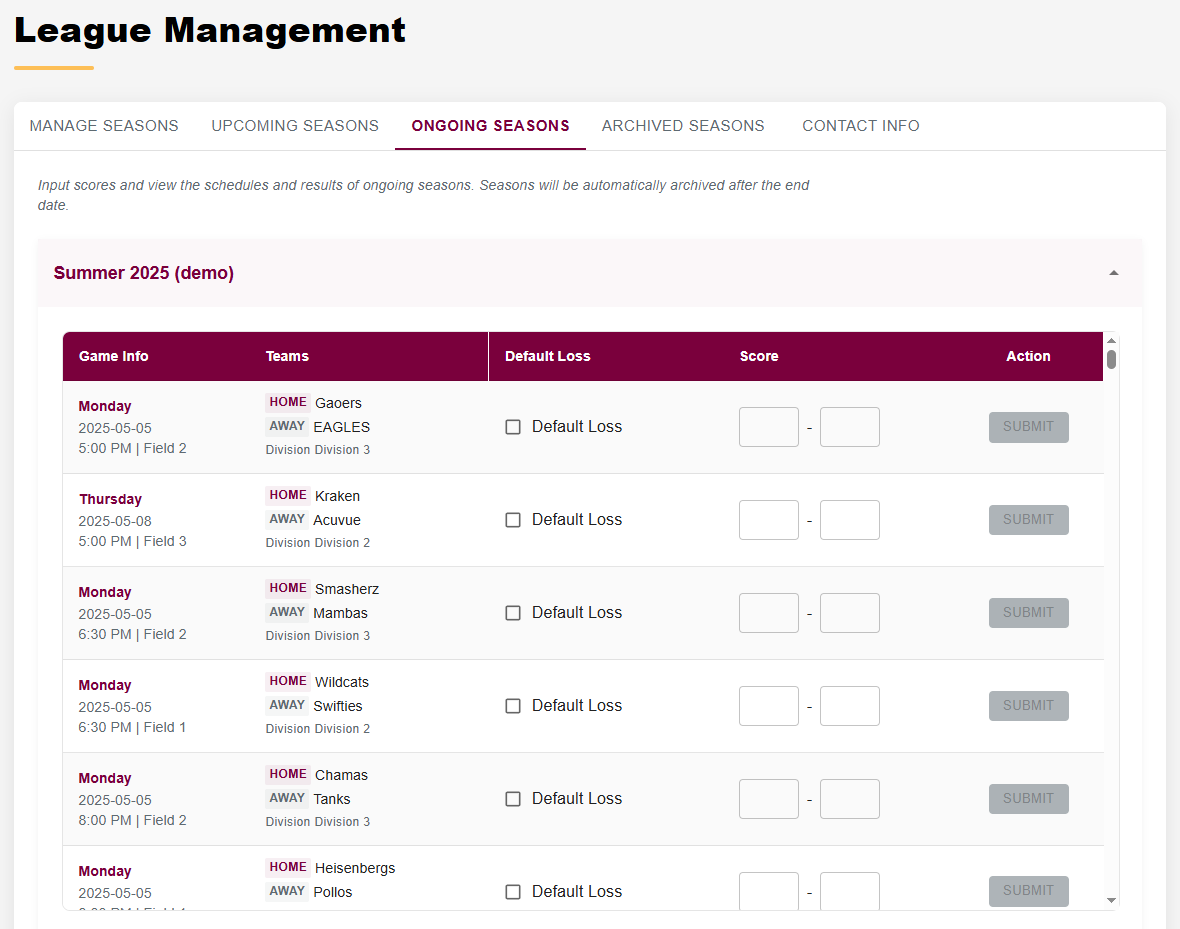
\includegraphics[width=1\textwidth]{ongoingseasons2.png}}
    \caption{In the ongoing seasons tab, the scores, schedules, and results can be viewed here}
\end{figure}

\begin{figure}[H]
    \centering
    \fbox{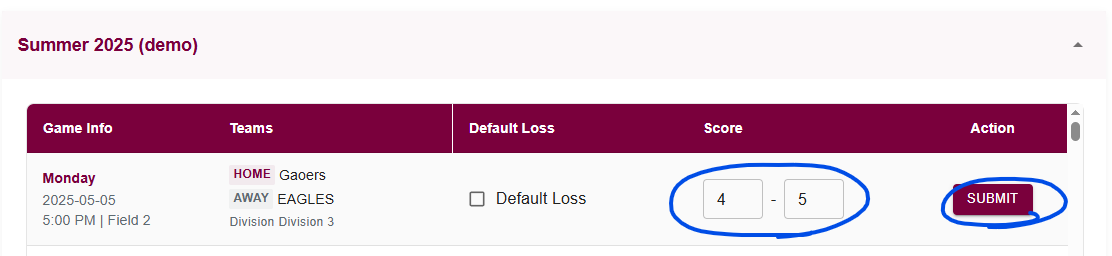
\includegraphics[width=1\textwidth]{ongoingseasons3.png}}
    \caption{You can change scores here by filling it out and clicking submit}
\end{figure}

\begin{figure}[H]
    \centering
    \fbox{
\includegraphics[width=1\textwidth]{ongoingseasons4.png}}
    \caption{You can also archive the season at the very bottom if needed}
\end{figure}

\subsection{Contact Info}
The commissioner can view contact information for team captains across all seasons.

\begin{figure}[H]
    \centering
    \fbox{
\includegraphics[width=1\textwidth]{contactinfo1.png}}
    \caption{Navigate to the manage view}
\end{figure}

\begin{figure}[H]
    \centering
    \fbox{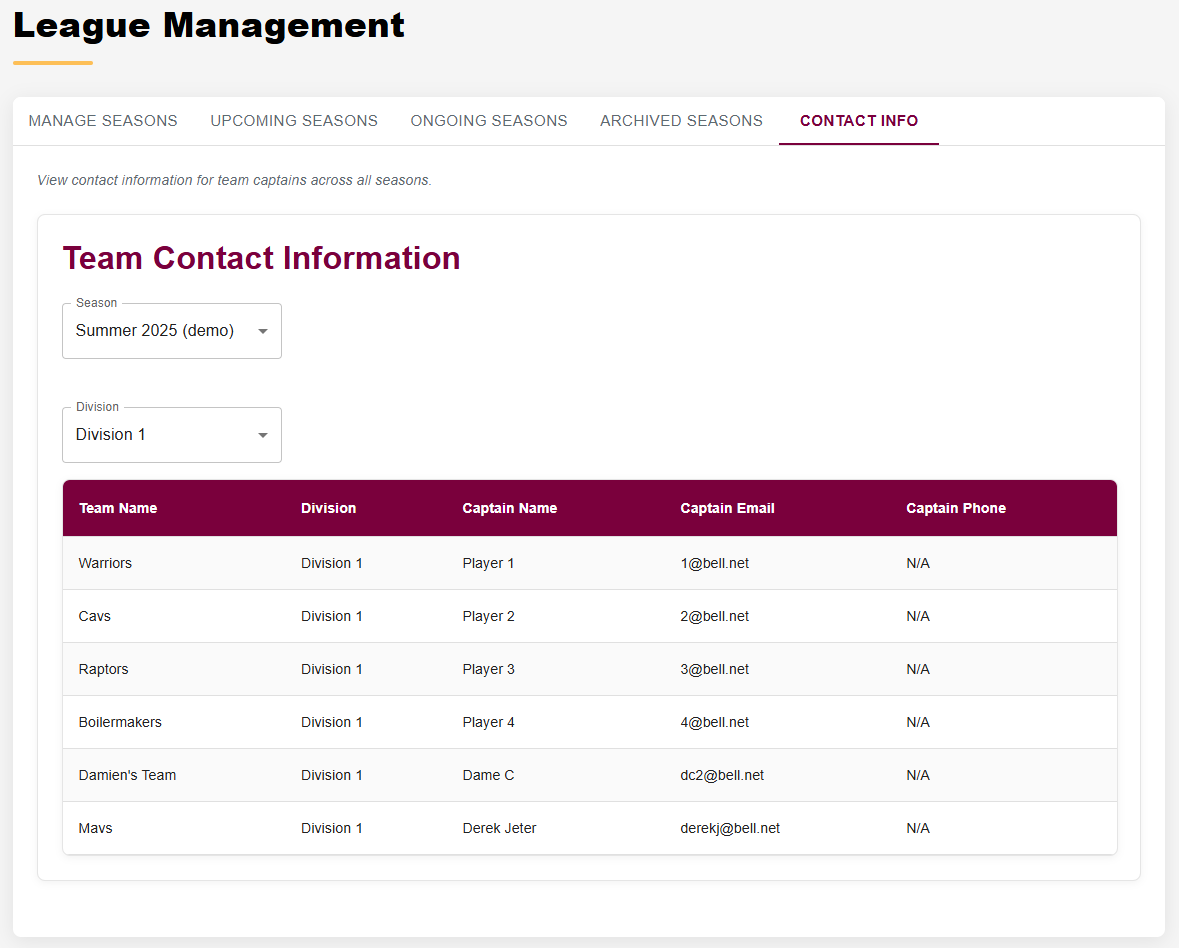
\includegraphics[width=1\textwidth]{contactinfo2.png}}
    \caption{In the contact info tab, the contact information of every team captain can be found}
\end{figure}




\section{FAQ}
The website also features an FAQ section that provides easy access to both the Player's Manual and Captain's Manual for quick reference. The section contains clear instructions and the very same visuals included in this user guide.

\section{Contact Information}
If there are any issues not listed here, please send an email to the commissioner at \texttt{neasej@mcmaster.com} or contact the original team who developed the platform.

\end{document}